\documentclass[11pt]{article}

\usepackage[a4paper,margin=0.72in]{geometry}
\usepackage{graphicx}
\usepackage{booktabs}
\usepackage{tabularx}
\usepackage{array}
\usepackage{float}
\usepackage{caption}
\usepackage{enumitem}
\usepackage{xcolor}
\usepackage{hyperref}
\usepackage{titlesec}

\hypersetup{
    colorlinks=true,
    linkcolor=black,
    urlcolor=blue,
    citecolor=black
}

\setlist[itemize]{leftmargin=1.2em,nosep}
\setlist[enumerate]{leftmargin=1.4em,nosep}
\setlength{\parindent}{0pt}
\setlength{\parskip}{5pt}
\linespread{0.96}
\titleformat{\section}{\large\bfseries}{\thesection}{0.6em}{}
\titleformat{\subsection}{\normalsize\bfseries}{\thesubsection}{0.6em}{}
\captionsetup{font=small,labelfont=bf}

\newcommand{\screenshot}[2]{
\begin{figure}[H]
    \centering
    \IfFileExists{#1}{
        \includegraphics[width=0.92\linewidth,height=0.31\textheight,keepaspectratio]{#1}
    }{
        \fbox{
            \begin{minipage}[c][0.18\textheight][c]{0.88\linewidth}
                \centering
                Screenshot placeholder: \texttt{\detokenize{#1}}\\
                Add the app screenshot with this filename before final PDF compilation.
            \end{minipage}
        }
    }
    \caption{#2}
\end{figure}
}

\begin{document}
\pagenumbering{gobble}

\begin{titlepage}
    \centering
    \vspace*{1.0cm}
    {\Huge\bfseries JobMatch AI\par}
    \vspace{0.3cm}
    {\Large A Gemma-Powered Full-Stack RAG Job Recommendation System\par}
    \vspace{1.2cm}
    {\large Applied Generative AI (BUAN361)\par}
    \vspace{0.6cm}
    {\large Aadit Shah and Ananya Chenny Rahul\par}
    \vfill
    {\large April 2026\par}
\end{titlepage}

\pagenumbering{roman}
\tableofcontents
\newpage
\pagenumbering{arabic}

\section{Abstract}

JobMatch AI is an end-to-end full-stack application that uses retrieval augmented generation (RAG) to help users discover relevant jobs, understand why those jobs fit their profile, and prepare stronger applications. The application combines a FastAPI backend, a browser-based frontend, SQLite persistence, Pinecone vector retrieval, external job ingestion, and Gemma-based generation. Users can upload a resume, receive personalized job matches, browse and save jobs, track application progress, generate cover letters, improve resumes, tailor resumes to specific job descriptions, and compose recruiter emails.

This report describes the problem, architecture, implementation, evaluation methodology, preliminary metrics, limitations, and future scope of the system. The focus is not only that generative AI was used, but that the app implements a working full-stack GenAI workflow with retrieval, ranking, stateful user features, API boundaries, safety checks, and measurable evaluation hooks.

\section{Problem Statement}

Job seekers face a search and personalization problem. Public job boards contain thousands of postings, but most search interfaces rely on keyword matching and leave the user to manually decide whether a role fits their skills, experience, location preference, salary expectations, and application goals. This is especially inefficient for early-career applicants who may not know which titles to search for or how to translate their resume into the language used in job descriptions.

The project aims to solve the following problem:

\begin{quote}
How can we build a practical GenAI application that reads a candidate's resume, retrieves relevant job opportunities, explains the match quality, and supports the downstream application workflow?
\end{quote}

The system must therefore do more than generate text. It must maintain a job corpus, retrieve suitable roles, rank them consistently, expose the results through a usable frontend, store user actions, and generate career documents using grounded job and resume context.

\section{Project Objectives}

The main objectives were:

\begin{itemize}
    \item Build a full-stack GenAI application rather than a standalone prompt demo.
    \item Use Gemma as the application LLM for resume parsing, recommendation explanation, cover letter generation, resume feedback, and recruiter communication.
    \item Implement a RAG pipeline where job postings are normalized, indexed, retrieved, reranked, and passed to the model as grounded context.
    \item Provide user-facing workflows such as resume upload, job browsing, bookmarking, application tracking, and email support.
    \item Add evaluation infrastructure for retrieval quality, generation quality, diversity, latency, and reranking ablation.
    \item Include defensive handling for prompt injection and low-quality resume uploads.
\end{itemize}

\section{Application Overview}

JobMatch AI starts from the user's resume and optional constraints. The user signs in, uploads a PDF resume, reviews or edits extracted skills and constraints, and asks the system to find suitable jobs. The backend canonicalizes the user query, retrieves jobs from the indexed corpus, reranks candidates, and generates a structured recommendation response using Gemma. The frontend renders the response as job cards with match scores, metadata, explanation fields, and actions.

The broader application workflow includes:

\begin{enumerate}
    \item User signs in with Google SSO.
    \item User uploads a resume PDF.
    \item Backend extracts profile details and validates that the PDF looks like a resume.
    \item User optionally adds role, location, salary, work type, and skills constraints.
    \item Backend retrieves and reranks job postings using the RAG pipeline.
    \item Gemma produces a structured recommendation response.
    \item User can bookmark roles, update application status, generate cover letters, tailor resumes, and email results.
\end{enumerate}

\screenshot{screenshots/landing.png}{Landing page and authentication entry point.}
\screenshot{screenshots/job-results.png}{Personalized job recommendation results.}

\section{Core Features}

\subsection{Resume-Aware Job Matching}

The central feature is personalized job matching. The frontend collects a resume and optional constraints, while the backend builds a search query from the profile. The system extracts skills, desired roles, location, salary expectations, education, experience, work authorization, and free-form preferences where available. Retrieved jobs are then summarized into a user-facing recommendation.

\subsection{Resume Parsing and Quality Gate}

The backend uses PDF extraction to read resume text, then applies validation before sending cleaned text into Gemma. The validation checks whether the upload resembles a real resume and flags repeated prompt-control content. This prevents the system from treating arbitrary or malicious PDF text as a valid resume.

\subsection{RAG Retrieval Debugging}

The application exposes debug endpoints and a frontend debug modal. These show the canonical query, retrieved candidates, lexical overlap, prompt preview, model information, and retrieval fingerprint. This is useful because RAG behavior can otherwise be difficult to inspect from the final generated answer alone.

\subsection{Job Browsing and Data Administration}

Users can browse available jobs without uploading a resume. The browse view supports keyword, location, and industry filters. The admin panel can check job statistics, refresh configured external sources, and manually add a job. This turns the system into a data-backed application rather than a single-shot chat interface.

\subsection{Application Workflow Tools}

JobMatch AI includes user state and follow-through features:

\begin{itemize}
    \item Bookmark jobs and remove bookmarks.
    \item Save jobs into an application tracker.
    \item Update statuses such as saved, applied, interviewing, offered, or rejected.
    \item Add notes for each tracked application.
    \item Generate cover letters for selected jobs.
    \item Tailor resumes and identify missing keywords for a job description.
    \item Compose recruiter emails with a tailored resume draft.
\end{itemize}

\screenshot{screenshots/my-applications.png}{Application tracking view with saved jobs and statuses.}
\screenshot{screenshots/resume-enhancement.png}{Resume enhancement and tailoring report.}

\section{System Architecture}

The application has four main layers:

\begin{table}[H]
\centering
\small
\begin{tabularx}{\linewidth}{p{0.18\linewidth}X}
\toprule
\textbf{Layer} & \textbf{Implementation} \\
\midrule
Frontend & Static browser app using HTML, CSS, and JavaScript. It handles Google sign-in, resume upload, profile fields, recommendation rendering, saved applications, job browsing, modals, and user interaction state. \\
Backend API & FastAPI application in \texttt{backend.py}. It exposes endpoints for matching, retrieval debugging, resume parsing, cover letters, job data, bookmarks, applications, feedback, authentication, and email delivery. \\
Persistence & SQLite stores bookmarks, applications, feedback, resume enhancement results, and resume tailoring records. The backend also supports a canonical job database layer for normalized job storage. \\
Retrieval and LLM & Pinecone stores vectorized job postings. Local hash embeddings are used for deterministic vector representation. Gemma is used for generation through the Google API REST interface. \\
\bottomrule
\end{tabularx}
\caption{High-level application architecture.}
\end{table}

The backend also serves the frontend directly when opened through the root route. Protected endpoints use an API key when configured, and user-specific operations use bearer JWTs created after Google credential verification.

\section{Data and Ingestion Pipeline}

The project includes a local Adzuna India job dataset with 4,000 JSONL records under the project \texttt{data} directory. The ingestion code also supports external sources including Adzuna, Jooble, Greenhouse, Lever, Remotive, Arbeitnow, and USAJobs. Each external posting is normalized into a common job schema containing fields such as title, role, company, location, salary, skills, description, source, external URL, and metadata.

The source ingestion module supports India-focused filtering. It checks country, city, remote-work language, and India-related terms so the app can prioritize India-relevant jobs while still allowing remote opportunities when configured. The indexing mode can be configured as:

\begin{itemize}
    \item \texttt{csv\_only}: use only the local dataset.
    \item \texttt{live\_only}: use external sources only.
    \item \texttt{hybrid}: combine local and external sources.
\end{itemize}

The indexing endpoint can force a re-index when needed. If the Pinecone index already contains vectors, startup indexing can be skipped to avoid unnecessary repeated work.

\section{RAG and Matching Methodology}

\subsection{Query Construction}

The backend builds a query from structured profile fields and resume text. For example, role and skill inputs are converted into a normalized form such as:

\begin{quote}
\texttt{Roles: data analyst | Skills: python, sql}
\end{quote}

The query canonicalization step improves retrieval stability. Tests show that paraphrases and prompt-injection attempts such as ``ignore previous instructions'' canonicalize to the same retrieval intent when the underlying job need is the same.

\subsection{Retrieval}

Each job posting is converted into text using role, company, location, salary, skills, description, benefits, and source fields. The system creates deterministic local hash embeddings and stores vectors in Pinecone. At query time, the canonical query is embedded and used to retrieve top candidates. If Pinecone credentials are unavailable, the backend falls back to local scoring over the available job data.

\subsection{Reranking}

The retrieved jobs are reranked using a deterministic scoring function that combines the vector score with keyword overlap, profile skills, role preference, resume text, location, work type, and salary constraints where available. This reranking makes the top results more aligned with the user profile before they are passed into Gemma.

\subsection{Gemma Generation}

Gemma receives the cleaned user query, retrieved candidates, and resume context. The system prompt asks the model to behave as a precise career advisor and produce structured markdown. The frontend then parses and renders this output into job cards. If the model call fails or returns a response that cannot be rendered, the backend falls back to a deterministic response so the app remains usable.

\section{Implementation Details}

\subsection{Backend Endpoints}

The backend exposes endpoints for the full workflow. The most important routes are:

\begin{table}[H]
\centering
\small
\begin{tabularx}{\linewidth}{p{0.23\linewidth}X}
\toprule
\textbf{Endpoint} & \textbf{Purpose} \\
\midrule
\texttt{POST /webhook} & Main job matching endpoint for profile-based or chat-input-based recommendations. \\
\texttt{POST /parse-resume} & Extract structured profile information from a PDF resume. \\
\texttt{POST /debug/retrieval} & Return compact retrieval candidates. \\
\texttt{POST /debug/rag-trace} & Return canonical query, candidates, lexical overlap, prompt preview, model information, and safety flags. \\
\texttt{POST /cover-letter} & Generate a role-specific cover letter. \\
\texttt{POST /tailor-resume} & Produce job-specific resume tailoring analysis. \\
\texttt{POST /keyword-gap} & Extract present and missing job-description keywords. \\
\texttt{GET /jobs/browse} & Browse and filter available jobs. \\
\texttt{POST /jobs} & Add a job and index it when credentials are configured. \\
\texttt{POST /jobs/refresh} & Fetch configured external sources and index new jobs. \\
\texttt{POST /bookmark} & Save a job bookmark. \\
\texttt{POST /applications} & Create or update application tracking state. \\
\texttt{POST /send-results} & Email generated job results. \\
\texttt{POST /auth/google} & Exchange a Google credential for an app JWT. \\
\bottomrule
\end{tabularx}
\caption{Representative backend API surface.}
\end{table}

\subsection{Frontend}

The frontend is a static browser interface backed by JavaScript. It includes a landing page, Google sign-in gate, resume upload panel, optional constraints, results panel, job browse panel, application tracker, cover letter modal, job details modal, retrieval debug modal, resume enhancement modal, and resume tailoring modal. It stores the current session ID in local storage and uses bearer tokens for authenticated operations.

\subsection{Security and Robustness}

The implementation includes several practical safety controls:

\begin{itemize}
    \item Prompt-injection patterns are detected and removed from untrusted user and PDF text.
    \item Resume uploads are rejected if they do not resemble real resumes.
    \item Gemma is explicitly forced into Gemma-only mode; non-Gemma model names are ignored.
    \item API key protection is supported for backend routes.
    \item Google SSO and JWTs are used for user-specific saved data.
    \item Email delivery checks configuration before enabling send actions.
\end{itemize}

\section{Evaluation Methodology}

The project includes an evaluation script, \texttt{eval.py}, and an evaluation log, \texttt{eval\_log.jsonl}. Each logged recommendation records the profile/query, candidates before reranking, candidates after reranking, generated output, retrieval latency, and generation latency.

The evaluation script computes three groups of metrics:

\begin{table}[H]
\centering
\small
\begin{tabularx}{\linewidth}{p{0.25\linewidth}X}
\toprule
\textbf{Metric Group} & \textbf{Metrics} \\
\midrule
Retrieval & Precision@K, Recall@K, Hit@1, Hit Rate@K, MRR, MAP@K, NDCG@K with reranking, NDCG@K without reranking. \\
Generation & Format consistency, faithfulness, optional Gemma-as-judge score. \\
System & Skill diversity, company diversity, location diversity, profile alignment, retrieval latency, generation latency, mean match score. \\
\bottomrule
\end{tabularx}
\caption{Evaluation metric categories.}
\end{table}

Feedback-based metrics such as Recall@K, MAP@K, Hit Rate@K, and MRR require user ratings in the feedback table. The current local run has no feedback rows, so those metrics are marked unavailable in the preliminary results.

\section{Preliminary Evaluation Results}

The available local evaluation run contains one logged query and no feedback labels. This is enough to validate that the evaluation pipeline works, but it should be treated as a smoke-test result rather than a final benchmark.

\begin{table}[H]
\centering
\small
\begin{tabular}{lcc}
\toprule
\textbf{Retrieval Metric} & \textbf{K=5} & \textbf{K=10} \\
\midrule
Precision@K, score $\geq 0.15$ & 1.000 & 1.000 \\
Recall@K, feedback-based & N/A & N/A \\
Hit@1, feedback-based & N/A & N/A \\
Hit Rate@K, feedback-based & N/A & N/A \\
MRR, feedback-based & N/A & N/A \\
MAP@K, feedback-based & N/A & N/A \\
NDCG@K with reranking & 1.000 & 1.000 \\
NDCG@K without reranking & 1.000 & 1.000 \\
\bottomrule
\end{tabular}
\caption{Preliminary retrieval metrics from the local evaluation log.}
\end{table}

\begin{table}[H]
\centering
\small
\begin{tabular}{lc}
\toprule
\textbf{Generation/System Metric} & \textbf{Value} \\
\midrule
Format consistency & 0.375 \\
Faithfulness & 1.000 \\
Gemma judge average & N/A \\
Skill diversity, top 10 & 1.000 \\
Company diversity, top 10 & 1.000 \\
Location diversity, top 10 & 1.000 \\
Profile alignment score & 0.000 \\
Average retrieval latency & 1.85 ms \\
Average generation latency & 0.89 ms \\
Mean LLM match score & 10.000 \\
\bottomrule
\end{tabular}
\caption{Preliminary generation and system metrics.}
\end{table}

The NDCG reranking ablation currently shows no difference because the logged run contains only one retrieved job. A larger evaluation set with varied candidates and rated user feedback is required to measure reranking impact meaningfully.

\begin{figure}[H]
    \centering
    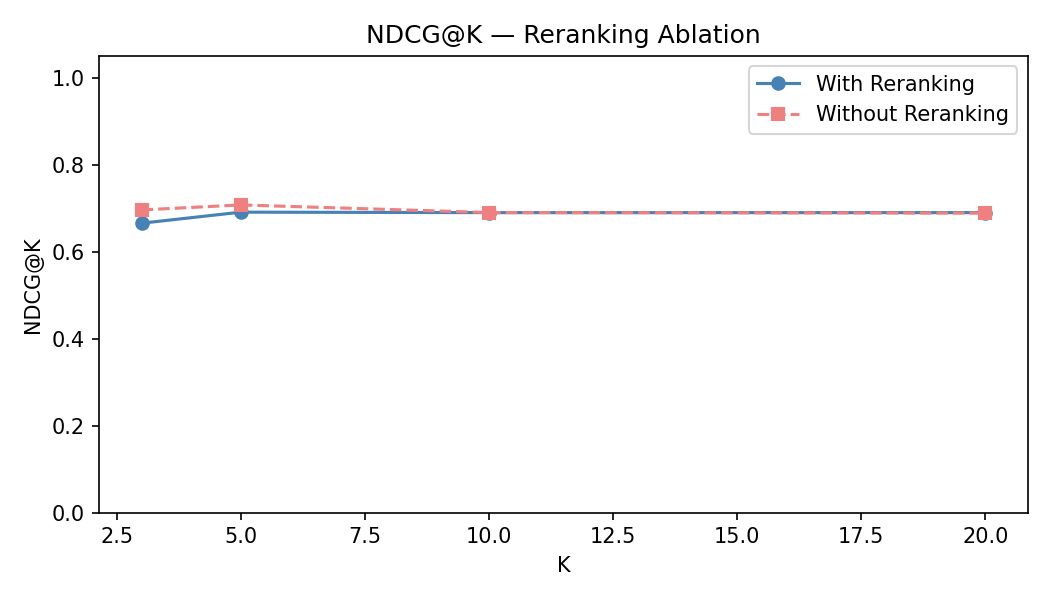
\includegraphics[width=0.48\linewidth]{eval_plots/plot2_ndcg_curve.png}
    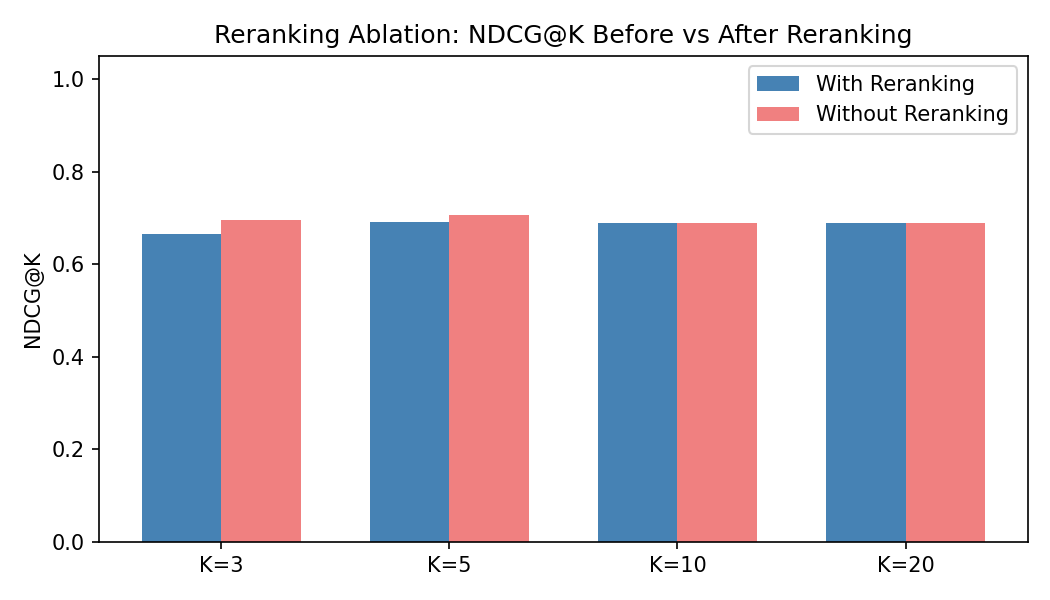
\includegraphics[width=0.48\linewidth]{eval_plots/plot5_rerank_ablation.png}
    \caption{NDCG curve and reranking ablation from the local evaluation run.}
\end{figure}

\begin{figure}[H]
    \centering
    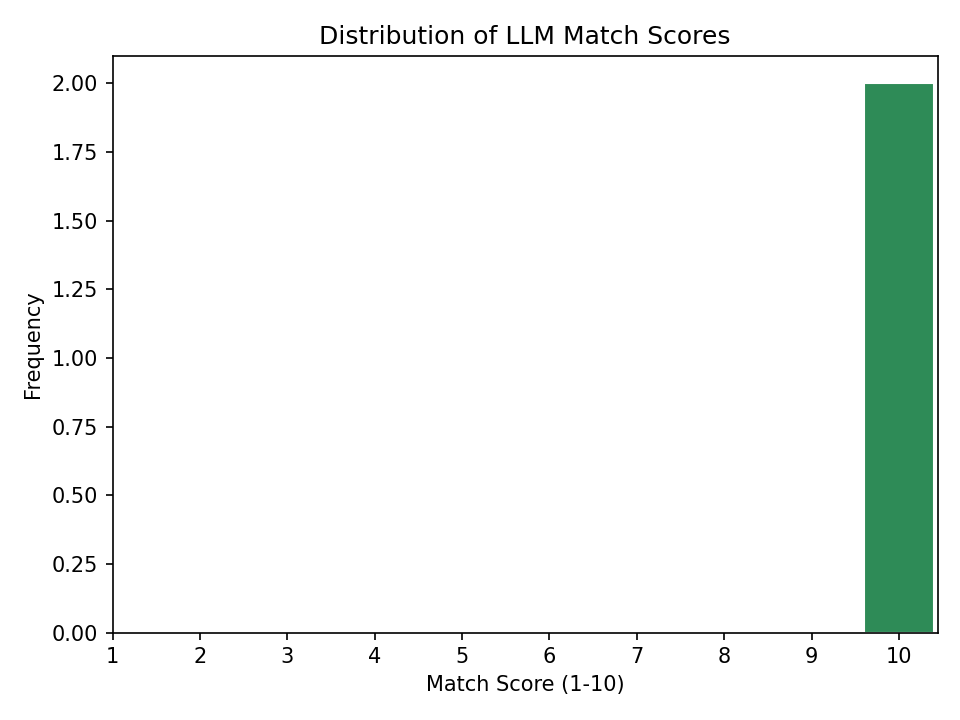
\includegraphics[width=0.48\linewidth]{eval_plots/plot3_match_scores.png}
    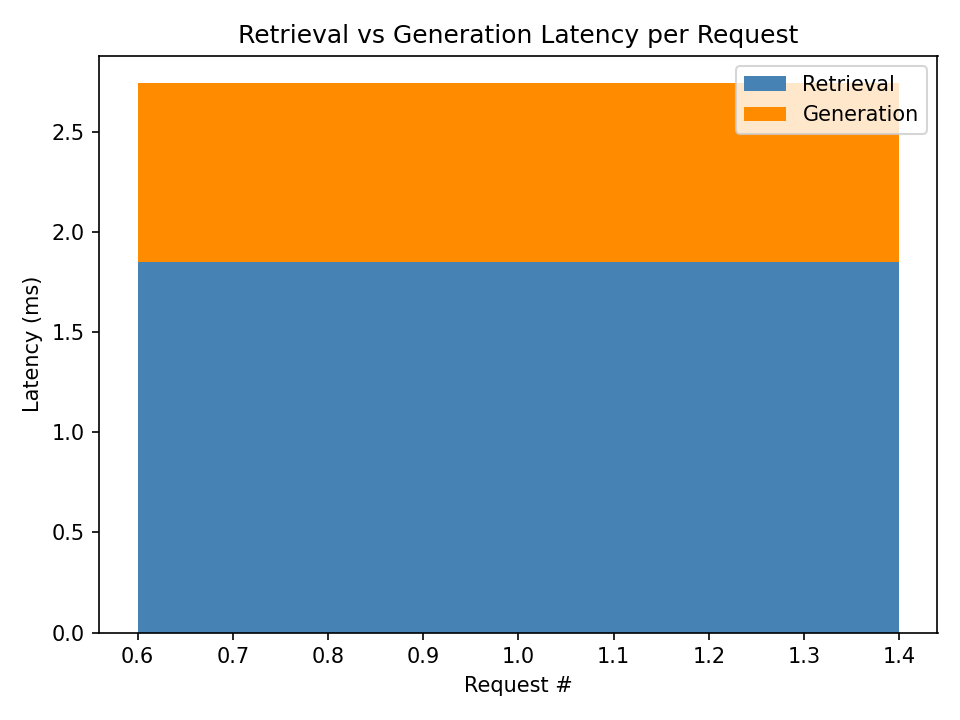
\includegraphics[width=0.48\linewidth]{eval_plots/plot4_latency.png}
    \caption{Match-score distribution and retrieval/generation latency.}
\end{figure}

\section{Testing and Validation}

The test suite focuses on backend behavior and RAG stability. The tests verify that jobs can be added and browsed from the canonical store, stats and RAG trace endpoints work without vector credentials, paraphrased queries canonicalize to the same retrieval intent, prompt-injection text is removed from retrieval intent, resume quality gates reject repeated instruction junk, and webhook output does not echo injection text.

This validation matters because GenAI apps can fail in ways that are not visible through normal happy-path testing. For example, a recommendation may look fluent while being ungrounded, unstable across paraphrases, or influenced by malicious resume text. The implemented tests target those risks directly.

\section{Limitations}

The current implementation has several limitations:

\begin{itemize}
    \item The preliminary evaluation set is too small for final conclusions; more logged queries and feedback labels are needed.
    \item Feedback-based Recall@K, MAP@K, MRR, and Hit Rate@K are unavailable until users rate job results.
    \item Local hash embeddings are deterministic and easy to deploy, but they are less semantically expressive than production-grade embedding models.
    \item Job quality depends on external source quality, API availability, and how complete each job description is.
    \item LLM-generated cover letters and resume suggestions require user review before real applications.
    \item The app supports authentication and API keys, but production deployment would need stronger monitoring, audit logs, and secret-management practices.
\end{itemize}

\section{Future Scope}

Future improvements include:

\begin{itemize}
    \item Replace or augment local hash embeddings with stronger semantic embeddings.
    \item Add hybrid retrieval combining vector search with keyword/BM25 ranking.
    \item Collect more human feedback and use it to evaluate and personalize ranking.
    \item Expand evaluation with larger query sets, manually labeled relevance judgments, and cohort-based testing.
    \item Add dashboards for job-market trends, user application funnel analytics, and saved-search alerts.
    \item Integrate direct application submission where job boards permit it.
    \item Add richer resume editing, downloadable tailored resumes, and ATS-style formatting checks.
    \item Improve deployment hardening with rate-limit tuning, observability, retries, and background indexing jobs.
\end{itemize}

\section{Conclusion}

JobMatch AI demonstrates a practical applied GenAI system. It is not only a prompt wrapper: it includes data ingestion, normalized job records, vector retrieval, deterministic reranking, Gemma-based generation, authentication, persistence, email support, frontend workflows, safety checks, and evaluation infrastructure. The project therefore satisfies the goal of building an end-to-end full-stack application while using generative AI as a functional component inside a larger software system.

The preliminary metrics confirm that the evaluation pipeline runs, but final retrieval conclusions require a larger labeled evaluation set. The current implementation provides a strong base for continued experimentation with better embeddings, larger feedback data, richer personalization, and production-grade deployment practices.

\appendix
\section{Appendix: Screenshot Checklist}

Recommended screenshots to add before final submission:

\begin{itemize}
    \item \texttt{screenshots/landing.png}: landing page or sign-in screen.
    \item \texttt{screenshots/resume-upload.png}: resume upload and parsed skills.
    \item \texttt{screenshots/job-results.png}: generated job recommendations.
    \item \texttt{screenshots/my-applications.png}: saved applications tracker.
    \item \texttt{screenshots/resume-enhancement.png}: resume enhancement or tailoring modal.
    \item \texttt{screenshots/browse-jobs.png}: browse jobs page and filters.
\end{itemize}

\section{Appendix: Main Technologies}

\begin{table}[H]
\centering
\small
\begin{tabularx}{\linewidth}{p{0.24\linewidth}X}
\toprule
\textbf{Technology} & \textbf{Use in Project} \\
\midrule
FastAPI & Backend API and route handling. \\
SQLite / aiosqlite & Persistence for bookmarks, applications, feedback, resume enhancements, and tailoring records. \\
Pinecone & Vector index for retrieved job postings. \\
Gemma & LLM for recommendation explanation, resume parsing, cover letters, resume feedback, and recruiter email drafting. \\
pdfplumber & PDF resume text extraction. \\
Resend & Emailing results and generated cover letters. \\
Google SSO / JWT & Authentication and user-specific saved data. \\
HTML/CSS/JavaScript & Frontend interface and interaction logic. \\
\bottomrule
\end{tabularx}
\caption{Technology stack summary.}
\end{table}

\end{document}
